\documentclass[a4paper]{article}
\usepackage{graphicx}
\usepackage{float}
\usepackage{amsmath}

\begin{document}

\section{Introduction}

The goal of this assignment is to create a control system for the attitude tracking problem of a Nadir pointing spacecraft. This control system is robust to external disturbances as well as noise and bias in the sensor measurements. To achieve this, the control system consists of a PD controller and a Multiplacative Quaternion Extended Kalman Filter (MQEFK). In order to further explore the problem space, additional goals were set beyond what were outlined in the assignment. Firstly, the code used simulate the satellite is written in Rust in order to gain an understanding of the practical challenges involved with writting production quality simulations software in a systems-level language. The code created for this assignment might not meet the bar of `production quality`, but a significant amount of understanding was gained in the attempt. Second, the LVLH frame of the circular orbit is modelled and the full Nadir tracking problem of aligning the body axes to the rotating LVLH reference frame is considered. Third, where ever possible quaternions are used to model the system in order to develop a deeper understanding about the math behind them. 

\section{Building the Model}

\subsection{Orbits and Reference Frames}

The Earth Centered Inertial (ECI) reference frame $\mathcal{F}_I$ is placed coincedent to the basis of the cartesian coordinates system. The position and velocty of the spacecraft w.r.t. $\mathcal{F}_I$ are defined by $\vec{r}$ and $\vec{v}$ respectivley. From this, the kinematics (\ref{eqn:kin_orbit}) and dynamics (\ref{eqn:dyn_orbit}) for a simple circular orbit can be written.

\begin{equation}
	\dot{r} = \frac{\vec{r} \times \vec{v}}{|\vec{r}|^2} \times \vec{r}
	\label{eqn:kin_orbit}
\end{equation}

\begin{equation}
	\dot{v} = \left|\frac{\vec{r} \times \vec{v}}{|\vec{r}|^2}\right|^2 \vec{r} 
	\label{eqn:dyn_orbit}
\end{equation}

The Local Vertical Local Horizon (LVLH) refernce frame $\mathcal{F}_{\textrm{LVLH}}$ can be built from these vectors by creating the quaternion $q_{LVLH}$ (\ref{eqn:q_lvlh}) that rotates $\mathcal{F}_I$ to $\mathcal{F}_{\textrm{LVLH}}$. This is done by creating a quaternion $q_1$ (\ref{eqn:q1}) that rotates the $\hat{k}$ vector of the basis to align with $\vec{r}$. A second quaternion $q_2$ (\ref{eqn:q2}) is then created to rotate the transformed basis about its $\hat{k}$ direction. The angle of this rotation is equal to the dot product of the transformed $\hat{i}$ direction and $\vec{v}$. Since the dot product operator provides no indication of the direction of rotation, only the magnitude, some logic is used to correctly rotate the basis.

\begin{equation}
	q_1 = [1 + \hat{k} \times -\hat{r}, [\hat{k} \times -\hat{r}]^T]^T
	\label{eqn:q1}
\end{equation} 

\begin{equation}
\begin{aligned}
	q2 &= \left[\cos\left(\frac{\theta}{2}\right), \left[\sin\left(\frac{\theta}{2}\right) * \hat{r}\right]^T\right]^T \\
	\theta &= \textrm{sign}\left(\sin^{-1}\left(\left[\left(q_1 * \hat{i} * q_1^{-1}\right) \times \hat{v} * \hat{r}^T\right] * \hat{i}\right)\right)\frac{\cos^{-1}\left(\left(q_1 * \hat{i} * q_1^{-1}\right) \circ \hat{v}\right)}{2} \\ \end{aligned}
	\label{eqn:q2}
\end{equation}

\begin{equation}
	q_{\textrm{LVLH}} = q_2 * q_1
	\label{eqn:q_lvlh}
\end{equation}

To determine correct functioning of the orbit, the LVLH frame transformation over time is simulated. This works thought theres is a discontinuity in the quaternion that pervents smooth control of the spacecraft over multiple orbits. This issues was not able to be solved within the time constraints of the project.

\begin{figure}
	\includegraphics[width=10cm]{images/lvlh_attitude.png}
	\caption{Evolution of $q_{\text{LVLH}}$ Over Time}
\end{figure}

\begin{figure}
	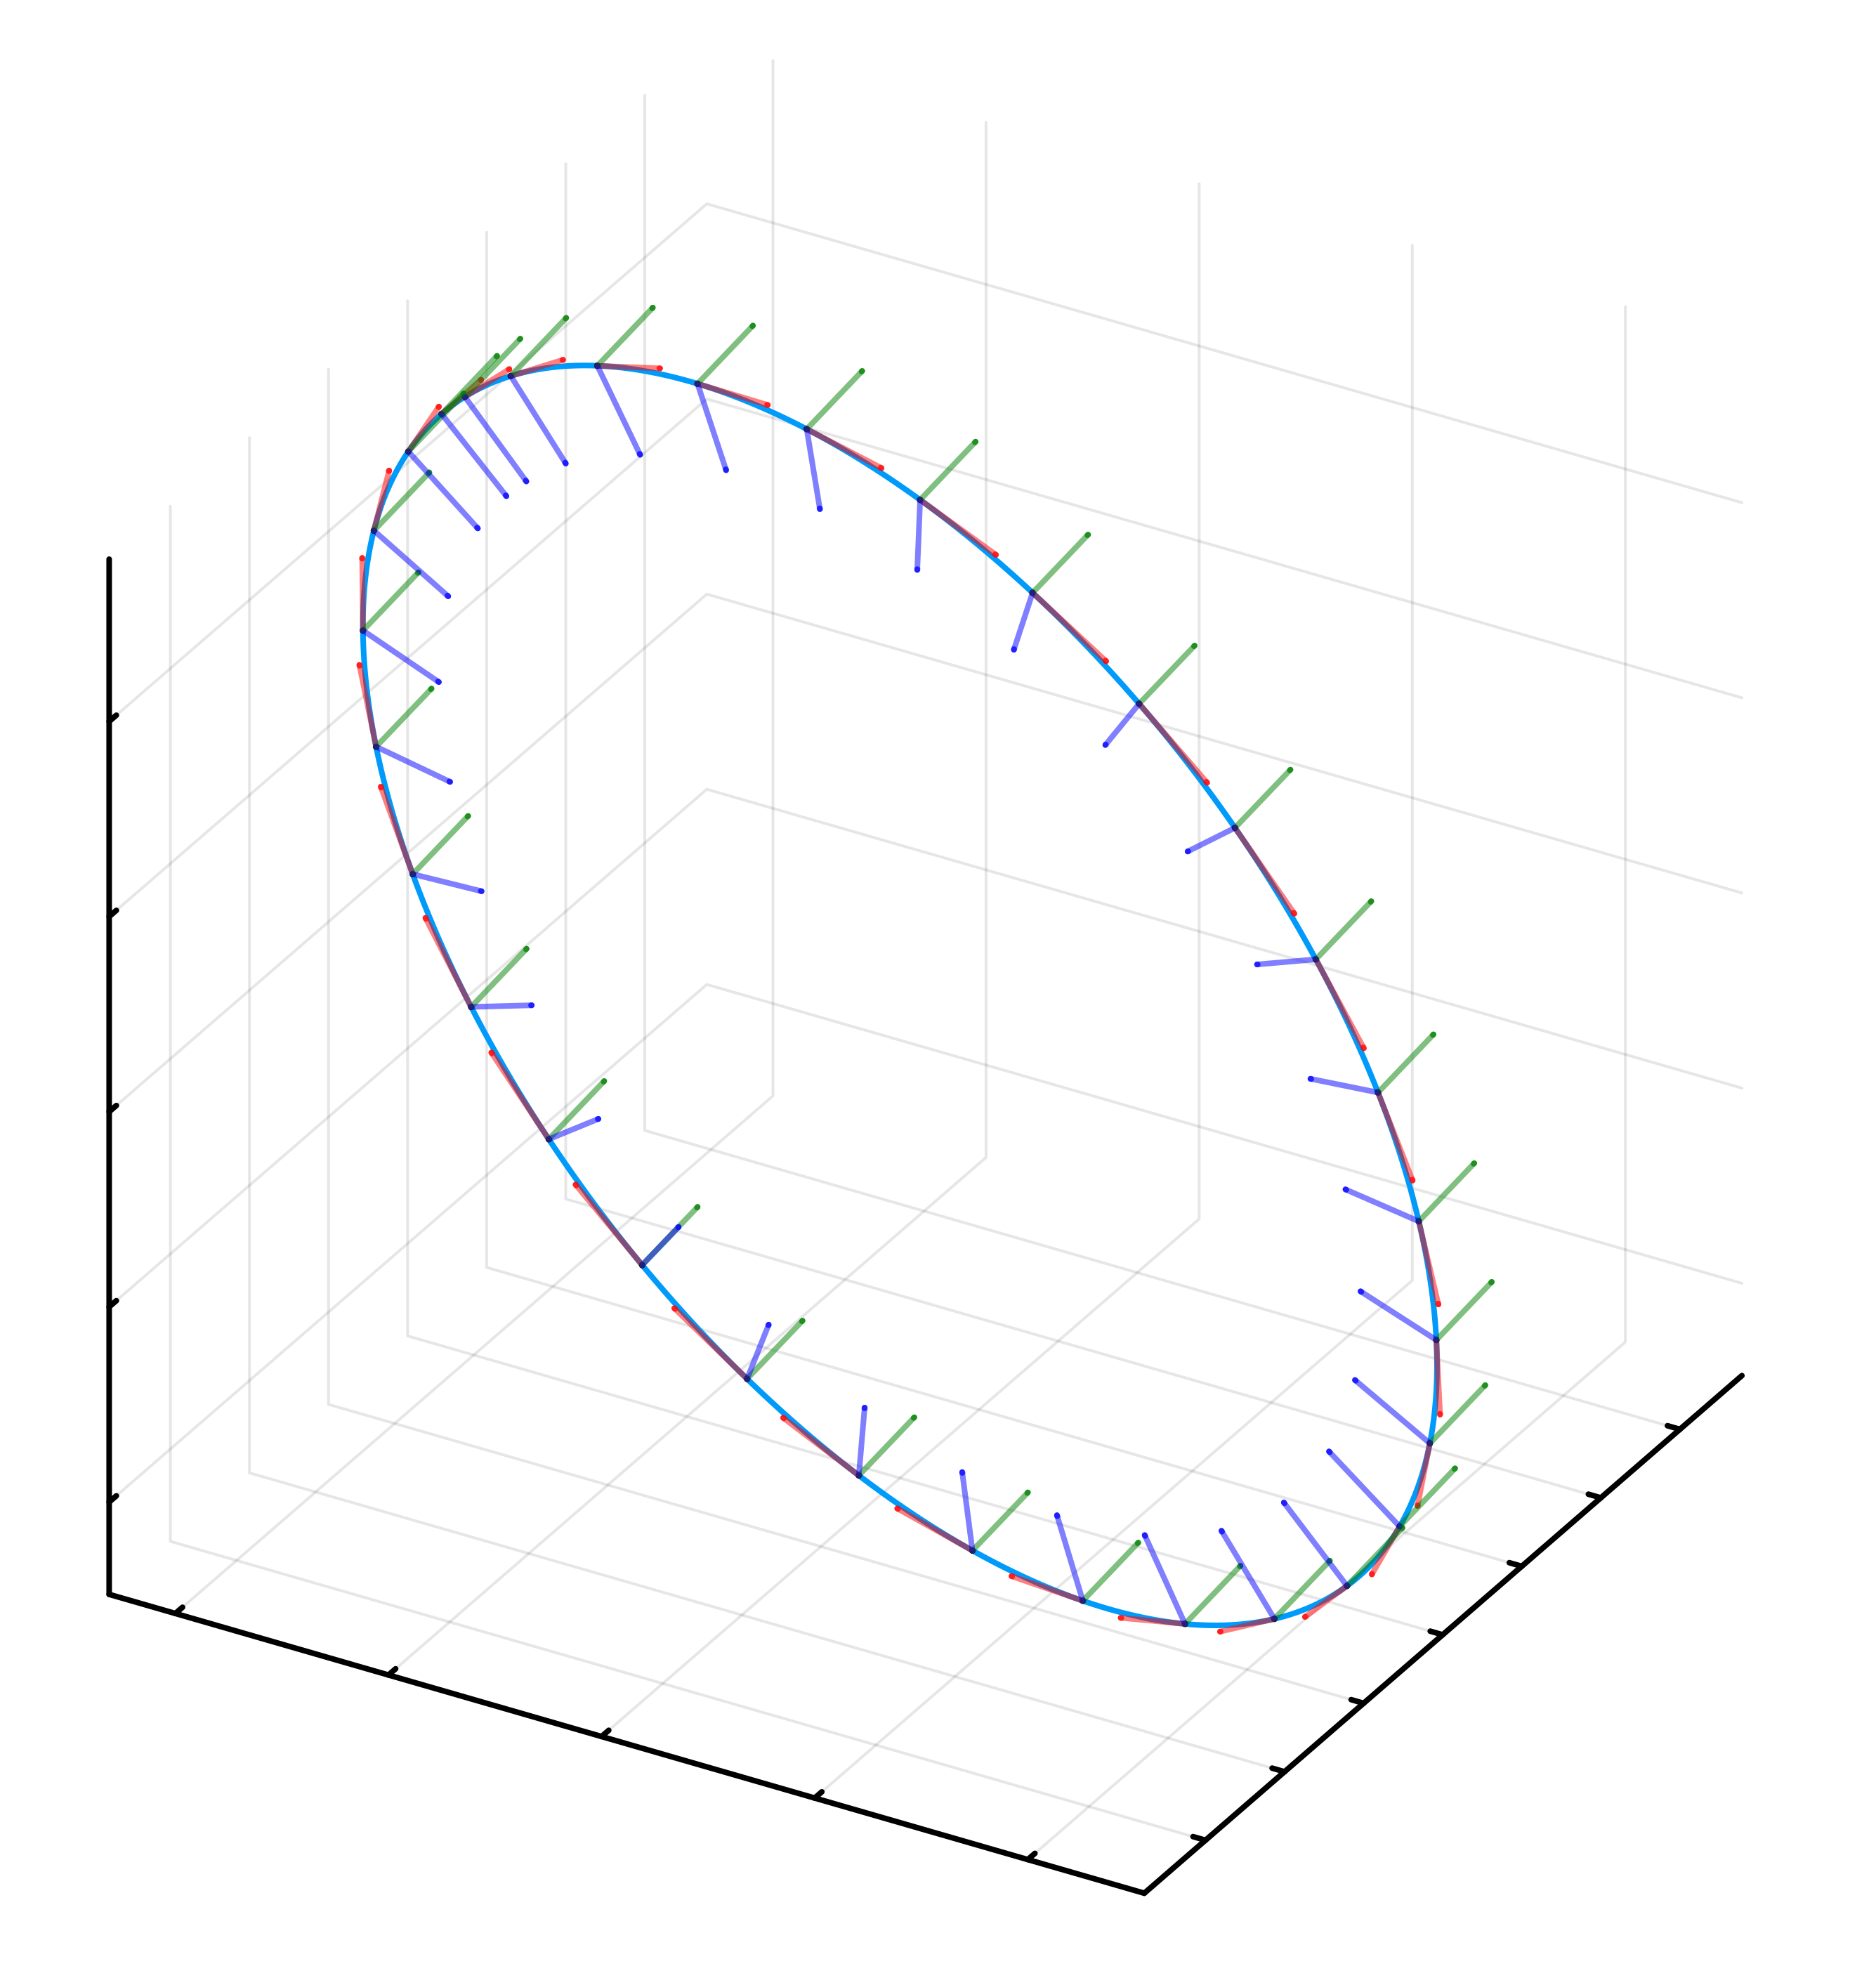
\includegraphics[width=10cm]{images/lvlh_orbit_0s_to_6100s.png}
	\caption{Evolution of $\mathcal{F}_{\text{LVLH}}$ Through One Orbit}
\end{figure}

\subsection{Sattelite Model}

\begin{equation}
	\dot{q}_{B/I} = \frac{1}{2} \omega_{B/I}^B * q_{B/I}
	\label{eqn:kin_sat}
\end{equation}

\begin{equation}
	\dot{\omega}_{B/I}^{B} = I^{-1} \left(-\omega_{B/I}^B \times I\omega_{B/I}^B + T_{gg} + T_{dist} + u\right)
	\label{eqn:dyn_sat}
\end{equation}

\begin{equation}
	I = \left[\begin{matrix}
		2500 & 0    & 0 \\
		0    & 2300 & 0 \\
		0    & 0    & 3100 \\
	\end{matrix}\right]
	\label{eqn:inertia}
\end{equation}

\begin{equation}
	T_{gg} = \frac{3\mu}{|\vec{r}|^3} -\hat{r} \times (-I\hat{r})
\end{equation}

\begin{equation}
	T_{dist} = \left[\begin{matrix}
		0.001 & 0.001 & 0.001
	\end{matrix}\right]
\end{equation}

\end{document}
